\documentclass[a4paper,11pt,spanish,sans]{exam}
\usepackage[spanish]{babel}
%\usepackage[utf8]{inputenc}
\usepackage{multicol}
%\usepackage[latin1]{inputenc}
\usepackage{fontspec}%la posta para las tildes con lualatex
\usepackage[margin=0.5in]{geometry}
\usepackage{amsmath,amssymb}
\usepackage{natbib}
\usepackage{graphicx}
\usepackage{hyperref}
\usepackage[usenames]{color}
%los de aca abajo capaz no los uso
\newcommand{\class}{Matemática: Guía de  Logaritmos}
\newcommand{\term}{2° Trimestre 2015}
\newcommand{\examnum}{Tema 1}
\newcommand{\examprof}{Alexis Gomel}
\newcommand{\examdate}{15/7/2015}
\newcommand{\timelimit}{60 Minutes}%no lo uso

%el header de las hojas.
\pagestyle{head}
\firstpageheader{}{}{}
\runningheader{\class}{\examnum\ - Page \thepage\ of \numpages}{\examdate}
\runningheadrule


\begin{document}


\noindent
\begin{tabular*}{\textwidth}{l @{\extracolsep{\fill}} r @{\extracolsep{6pt}} l}
\textbf{\class} & \textbf{Profesor: \examprof}\\

%\textbf{Time Limit: \timelimit} & Teaching Assistant & \makebox[2in]{\hrulefill}
\end{tabular*}\\
\rule[2ex]{\textwidth}{2pt}


{{\small Esta guía es simplemente una guía. \textbf{\underline{NO} reemplaza ni incluye todo el material que se da en clase}}}.

\begin{center}
	\section*{Guía de Logaritmos}
\end{center}


%%%%%%%%%%%%%%%%%%%%%%%%%%%%%%%%%%%%%%%%%%%
\section*{Algunos ejemplos graficos de Logaritmos}

Definición de logaritmo: $y=log_a(x)$ $\iff$ $a^{y}=x$.

Ejemplo: $8^2=64$ $\iff$ $2=log_8(64)$

\begin{figure}[h!]
\centering
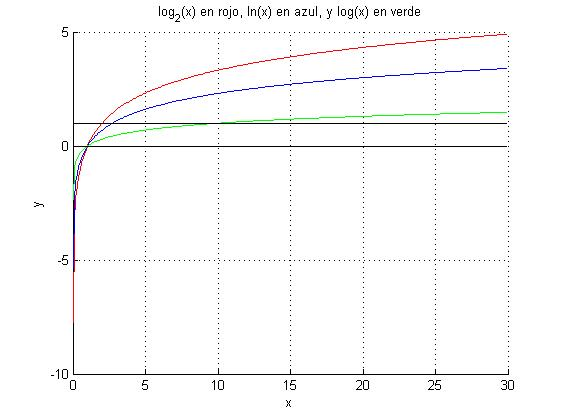
\includegraphics[width=0.6\textwidth]{compararlogs.jpg}
\caption{$log(x)$ en verde, $log_2(x)$ en rojo  y $ln(x)$ en azul.}
\label{fig:coplogs}
\end{figure}

\begin{figure}[h!]
\centering
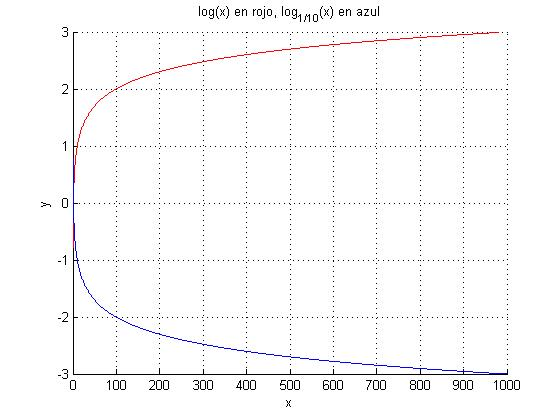
\includegraphics[width=0.6\textwidth]{amboslog10.jpg}
\caption{Graficos de $log(x)$ y $log_{\frac{1}{10}}(x)$.}
\label{fig:amboslogs}
\end{figure}\\

Si se traban con algún ejercicio, pasen al siguiente, y vuelvan al ejercicio difícil mas tarde.

\section{Resolver:}
\begin{enumerate}
\begin{multicols}{2}
\item $log_2(\frac{1}{128})$
\item $5^{4.log_5(2)}$
\item $4^{log_4(2)+log_4(7)}$
\item $log_3(\sqrt[5]{27}) $
\item $10^{2.log(5)}$ 
\item $e^{3.ln(4)-2.ln(3)+10^{28}.ln(1)}$
\item $a^{b.log_a(c)}$
\item $log_b(log_a(a^{(b^k)}))$
\item $a^{log_a(b)+log_a(d)-h.log_a(c)}$
\item $log_a(b)-log_a(c)=0$

\columnbreak

Sabiendo que $log_2(5) \simeq 2,3$, calcular:

\item $log_2(10)$
\item $log_2(2,5)$
\item $log_2(\sqrt(5))$
\item $log_2(25) $\\
Cambio de base:

\item $log_5(2)$
\item $log_{a^n}(a^{m})$
\item $log_2(\sqrt{5})$
\end{multicols}
\end{enumerate} 



\section{Graficos:}
Graficar Las siguientes funciones (basta con usar solo 4 puntos):

\begin{enumerate}%cambiar funcion
\item $log_3(3.(x+3))$

\item $log_{1/2}(4.(x-1))$

%elegir otro ejemplo, capaz el del examen, asi lo tiene visto.
\item Encontrar $a$ y $b$  a partir del gráfico de $y=log_a(x-b)$
\begin{figure}[h!]
\centering
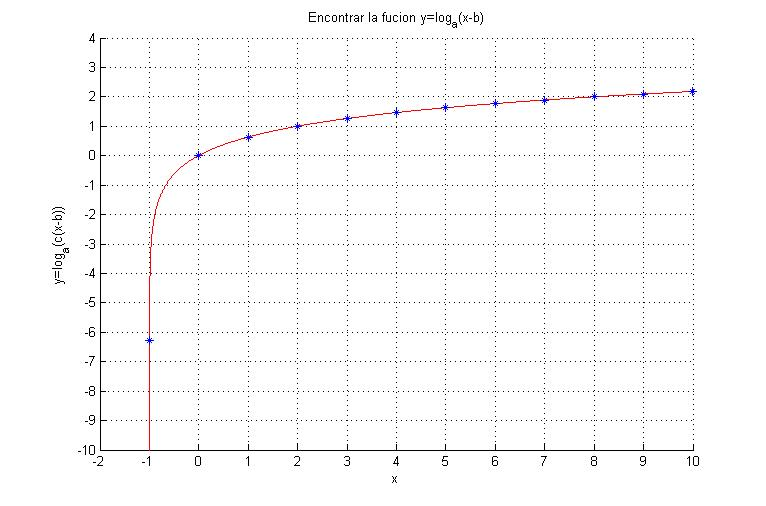
\includegraphics[width=0.55\textwidth]{encontrarlog3xmas1.jpg}
\caption{Encontrar $a$,$b$ y $c$,  a partir del gráfico de $y=log_(a)(x-b)$.
Los asteriscos azules marcan el valor de $y$ para $-1.00001, 2 , 3, 4, 5, 6...$}
\label{fig:logaritmo}
\end{figure}
\end{enumerate}

\section{Encontrar, si es posible, el valor de x :}

\begin{enumerate}
\begin{multicols}{2}

\item $log(x)=3.log(2)$
\item $log_2(3x+4)=1$
\item $10.log_5(x)-5.log_5(x)-5=0$%ojo con este a ver si sale o no.
\item $log_3(x^2)+log_3(x)-6=0$
\item $2^{x+1}-5.2^{x}+3=0$

\columnbreak

\item $2^x+2^{x+1}+\frac{5}{4}2^{x-2}=256$
\item $-3^x+4.3^{x+1}=99$
\item $3.log_2(x)-2.log_4(x)=2$
\item $log(x^2-3x+12)=1$

\end{multicols}
\end{enumerate}

\section{Uso de la calculadora}
Usando la calculadora, uno puede calcular el $log(x)$ y $ln(x)$, para cualquier numero. Sabiendo esto, calcular $x$ :


\begin{multicols}{2}
Usando $log(x)$ :

\begin{enumerate}
\item  $ 3^{x}.5^{2x}=4 $

\item  $ log_7(28) $

\columnbreak 

Usando $ln(x)$:

\item $log_8(5)$

\item $\frac{1}{3}^{x}.4^{\frac{x}{2}}=3$
\end{enumerate}
\end{multicols}
\\

\section{Ejemplo de Aplicación}
La población de una ciudad se triplica cada $50$ años. En el tiempo $t = 0$ , esta población es de $100000$ habitantes. Por lo tanto la población a lo largo del tiempo se puede expresar como $P(t)=10000.3^{\frac{t}{50}}$
cuál es la población después de 
a) 100 años? 
b) 150 años? 
c) 200 años? \\


\rule[2ex]{\textwidth}{2pt}


Observación: Para saber si hiciste bien un ejercicio, acordate de la definición de logaritmo, y exponencia el resultado que obtuviste, o reemplaza por tu valor de x.



\section*{Extra}

%El numero $e\simeq$ ..  breve bio de euler-
\begin{itemize}
\item Para tener una idea practica de que tan lento crece $log(x)$, busquen "Powers of ten" en youtube, un vídeo que muestra cuanto cambian las cosas que vemos a medida que consideramos cuadrados de $10^x $ metros de lado. Por ejemplo, un cuadrado de $10m$ ($log(10)=1$) de lado es algo de un tamaño normal para  un humano(una habitación, por ejemplo), mientras que en un cuadrado de $10^7$ metros ($log(10^7)=7$), es del tamaño del planeta tierra, y el $log(x)$ solo cambio 6 números!.
También pueden verlo de mantera interactiva en la pagina \href{www.scaleofuniverse.com}{\textcolor{blue}{www.scaleofuniverse.com}}  .

\item Al que le interese, la pagina http://www.librosmaravillosos.com/grandesmatematicos/capitulo09.html tiene una biografía muy interesante sobre  Leonhard Euler (1707-1783), el que le puso 'e' al numero e entre muchas otras cosas, uno de los matemáticos mas importantes de la historia. Para que tengan una idea,  Euler era tan groso que le daba clases a la Princesa Catalina de Rusia, que lo trataba como a un noble; y cuando se quedo ciego le dictaba sus trabajos a sus hijos, e incluso se volvió mas prolifero como matemático que cuando tenia la vista. 

\item There is a theory which states that if ever anyone discovers exactly what the Universe is for and why it is here, it will instantly disappear and be replaced by something even more bizarre and inexplicable.
There is another theory which states that this has already happened.[Douglas Adams. The Hitchhiker's Guide to the Galaxy.]%\citep{adams1995hitchhiker}

\centering
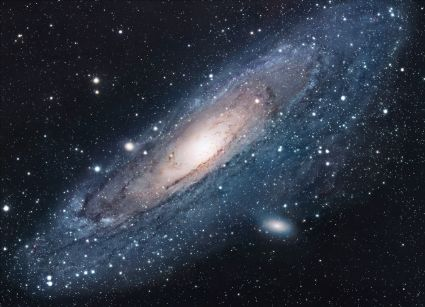
\includegraphics[scale=1.3]{universe.jpg}\\
\caption{The Universe}
\label{fig:univerise}


\end{itemize}

%\bibliographystyle{plain}
%\bibliography{references}


%
%\section*{Resultados}
%\begin{enumerate}
%\item
%\begin{enumerate}
%\item -7 ; \item 16 ; \item .. ; \item $3/5$ ; \item 25 ; \item $64/9$ ; \item $c^b $ ;\item $k$ ;\item $\frac{b.d}{c^h} $  ;\item $b=1/c$ ;\item  $2.2,3$ ;\item $2-2,3 = 0,3$ ;\item 2,3/2 ;\item  4,6 ;\item 1$/2,3$ ;\item m/n ;\item  ; 
%\end{enumerate}
%
%\item 
%\begin{enumerate}
%\item
%\item
%\item $log_3(x+1)$
%\end{enumerate}
%
%\item
%\begin{enumerate}
%\item $x=8$
%\item $-2/3$
%\item $x=5$
%\item $x=9$
%\item 
%\item 
%\item $x=2$
%\item $x=2$
%\item $x=1$,$x=$ 
%\end{enumerate}
%
%\item
%
%\item 
%
%
%\end{enumerate}


%%ejercicios extra:
%\item $5^{x+2}-10.5^x=900$
%\item $log_3(x+\sqrt{5})+log_3(x-\sqrt{5})=2$
%\item $e^{3.ln(3) + 2.ln(5) - 2^{6}.ln(1)}$
%\item $log_{b^m}(b^n)$

\end{document}